\documentclass[12pt]{article}
\usepackage{graphicx} % Required for inserting images
\usepackage[parfill]{parskip}
\usepackage{verbatimbox}
\usepackage{fancyvrb}
\usepackage{exercise}
\usepackage{hyperref}
\usepackage{csquotes}

% Palatino for main text and math
\usepackage[osf,sc]{mathpazo}

% Helvetica for sans serif
% (scaled to match size of Palatino)
\usepackage[scaled=0.90]{helvet}

%
%
\makeatletter
\@ifundefined{lhs2tex.lhs2tex.sty.read}%
  {\@namedef{lhs2tex.lhs2tex.sty.read}{}%
   \newcommand\SkipToFmtEnd{}%
   \newcommand\EndFmtInput{}%
   \long\def\SkipToFmtEnd#1\EndFmtInput{}%
  }\SkipToFmtEnd

\newcommand\ReadOnlyOnce[1]{\@ifundefined{#1}{\@namedef{#1}{}}\SkipToFmtEnd}
\usepackage{amstext}
\usepackage{amssymb}
\usepackage{stmaryrd}
\DeclareFontFamily{OT1}{cmtex}{}
\DeclareFontShape{OT1}{cmtex}{m}{n}
  {<5><6><7><8>cmtex8
   <9>cmtex9
   <10><10.95><12><14.4><17.28><20.74><24.88>cmtex10}{}
\DeclareFontShape{OT1}{cmtex}{m}{it}
  {<-> ssub * cmtt/m/it}{}
\newcommand{\texfamily}{\fontfamily{cmtex}\selectfont}
\DeclareFontShape{OT1}{cmtt}{bx}{n}
  {<5><6><7><8>cmtt8
   <9>cmbtt9
   <10><10.95><12><14.4><17.28><20.74><24.88>cmbtt10}{}
\DeclareFontShape{OT1}{cmtex}{bx}{n}
  {<-> ssub * cmtt/bx/n}{}
\newcommand{\tex}[1]{\text{\texfamily#1}}	% NEU

\newcommand{\Sp}{\hskip.33334em\relax}
\newcommand{\NB}{\textbf{NB}}
\newcommand{\Todo}[1]{$\langle$\textbf{To do:}~#1$\rangle$}

\EndFmtInput
\makeatother
%

% Bera Mono for monospaced
% (scaled to match size of Palatino)
% \usepackage[scaled=0.85]{beramono}

\title{What does it take to be a hero? and other questions from statistical mechanics.}
\author{Dan Piponi}
\date{September 2024}

\begin{document}

\maketitle

\section{We only hear about the survivors}
In the classic Star Trek episode \emph{Errand of Mercy}, Spock computes the chance of success:
\begin{displayquote}
CAPTAIN JAMES T. KIRK : What would you say the odds are on our getting out of here?

MR. SPOCK : Difficult to be precise, Captain. I should say, approximately 7,824.7 to 1.
\end{displayquote}
And yet they get out of there. Are Spock's probability computations unreliable?
Think of it another way. The Galaxy is a large place.
There must be tens of thousands of Spocks, and Grocks, and Plocks out there on various missions.
But we won't hear (or don't want to hear) about the failures.
So they may all be perfectly good at probability theory, but we're only hearing about the lucky ones.
This is an example of survivor bias.

\section{Simulation}
We can model this.
I've written a small battle simulator for a super-simple made up role-playing game.
Our intrepid wannabe hero has to battle a monster with way more hit points.
Only very few will survive, but survivor will return home with an unlikely sounding story to tell.

To find out about that story I record some of the die rolls.
In my rules, each time the warrior hits they do 1d8 damage.
But when we look at the results for the 6 in a million that survive, the distribution of damage rolls is skewed upwards.
Although a priori we expect $P(1)=P(2)=\ldots=P(8)=\frac{1}{8}$, when we condition on surviving we
get the table
\begin{center}
\begin{tabular}{|c|c|c|c|c|c|c|c|c|}
\hline
Roll & 1 & 2 & 3 & 4 & 5 & 6 & 7 & 8\\
\hline
Probability & 0.069 & 0.0806 & 0.094 & 0.111 & 0.127 & 0.147 & 0.172 & 0.198\\
\hline
\end{tabular}
\end{center}
which I also plot in Figure~\ref{rolls:1}.
This corresponds to a mean of $5.27$, quite a bit higher than $4.5$.

\begin{figure}
\begin{center}
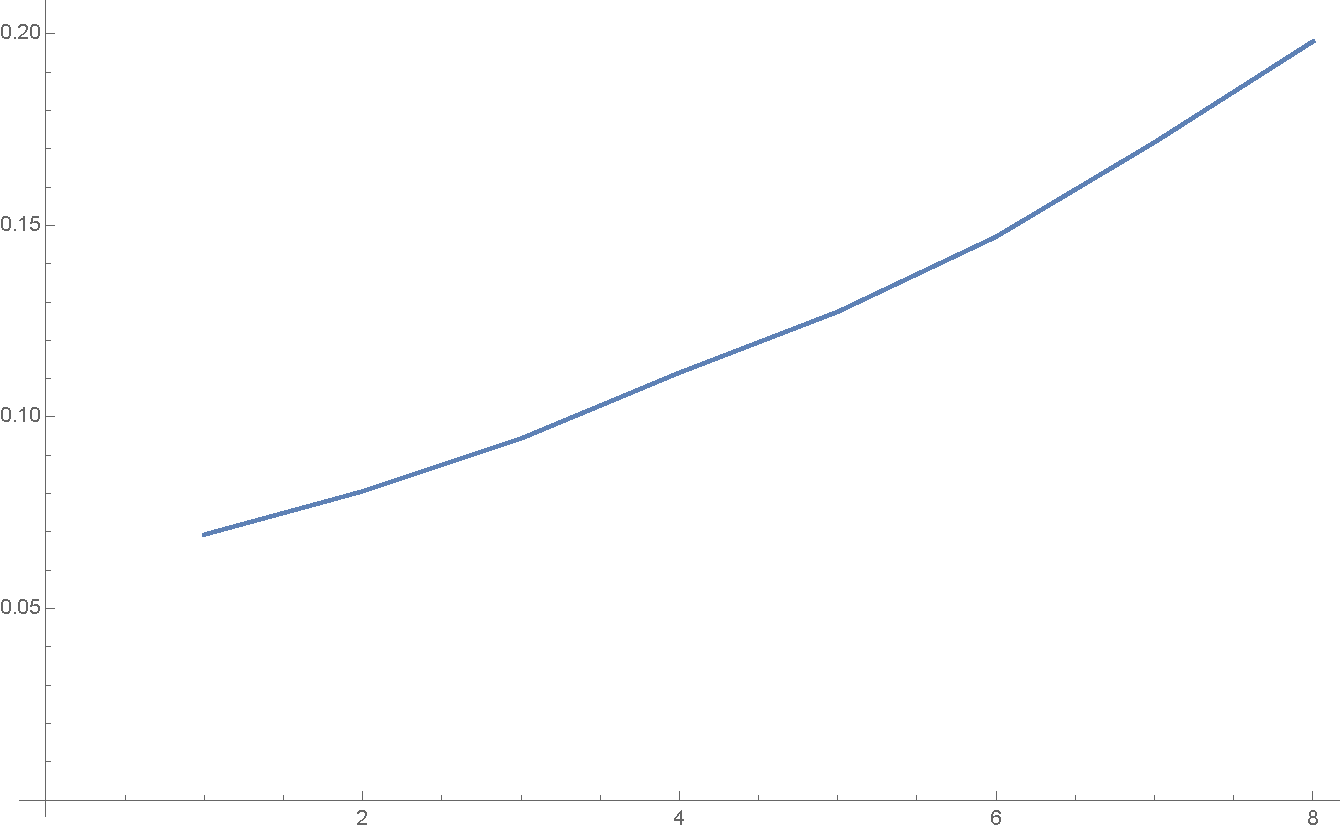
\includegraphics[scale=0.5]{rolls1.pdf}
\caption{Frequency of damage rolls}
\label{rolls:1}
\end{center}
\end{figure}

The distribution is significantly skewed upwards.
To surviving fighters this is how the world looks - it seems like it's a feature of the world that when you roll d8, you're much more likely to get 8 than 1.
(This must be how the world looks to most billionaires too.)

But look closely at the graph and there's something more going on: the graph has a slight convexity.
We can explain that too, and here we veer slightly towards statistical physics.

Let's use a simplified model. Suppose we roll 100d8. We expect a mean of 450.
Lets say we get 527, which closely matches our experiment above.
We can now ask for the conditional distribution of each die roll given that the sum is 527.
I'll use Mathematica.
Define \verb|num[s,n,m]| to be the number of ways to roll a total of $s$ using $n$ $m$-sided dice:

\begin{verbatim}
num [s_, n_, m_] := Sum[
     Module[
       {k = s - n - m r},
          (-1)^r
           Binomial[n, r] Binomial[n + k - 1, k]],
           {r, 0, Quotient[s - n, m + 1]}]
\end{verbatim}

And now we can use Bayes' theorem to tabulate the probabilities of each roll, $i$, by counting how many ways we can score a total of $527-i$ using 99 dice:

\begin{verbatim}
w = Table[num[527 - i, 99, 8], {i, 1, 8}];
N[w/Total[w]]
\end{verbatim}

We get
\begin{center}
\begin{tabular}{|c|c|c|c|c|c|c|c|c|}
\hline
Roll & 1 & 2 & 3 & 4 & 5 & 6 & 7 & 8\\
\hline
Probability & 0.069 & 0.0808 & 0.094 & 0.110 & 0.128 & 0.148 & 0.172 & 0.198\\
\hline
\end{tabular}
\end{center}
These probabilities are very close to our empirical numbers so I think we have a pretty good explanation for our results.

\section{Maximum entropy}
But there's another way to approximate this using one of my favourite papers:
\href{https://purl.stanford.edu/kr402kg0888}{Maximum Entropy and Conditional Probability} by Campenhout and Cover.
The idea there is that the maximum (relative) entropy distribution is a conditional distribution, and vice versa.
That paper really helped me understand max entropy.
Using the idea of that paper we want to find the maximum entropy distribution on $\{1,2,\ldots,8\}$ consistent with having a mean matching ours of $0.527$.
I'll leave it as an exercise in calculus and Lagrange multipliers to show that this means the probability of rolling $i$ is given by $a\exp(-bi)$ for some choice of $a$ and $b$.
Again we can use Mathematica:

\begin{verbatim}
s = Solve[{Sum[a Exp[-b i], {i, 1, 8}] == 1, 
    Sum[i a Exp[-b i], {i, 1, 8}] == 5.2654, a \[Element] Reals, 
        b \[Element] Reals}, {a, b}];
        u = Table[a Exp[-b i] /. s[[1]], {i, 1, 8}]
\end{verbatim}
and we get
\begin{center}
\begin{tabular}{|c|c|c|c|c|c|c|c|c|}
\hline
Roll & 1 & 2 & 3 & 4 & 5 & 6 & 7 & 8\\
\hline
Probability & 0.070 & 0.081 & 0.094 & 0.109 & 0.127 & 0.148 & 0.171 & 0.198\\
\hline
\end{tabular}
\end{center}

In Figure~\ref{rolls:2} I plot the simulation results and the max entropy distributions together so you can see how similar they are.
I also plot a straight line distribution with the same mean so you can see it is not a good model.

\begin{figure}
\begin{center}
\includegraphics[scale=0.5]{Rolls2.png}
\caption{Three distributions compared}
\label{rolls:2}
\end{center}
\end{figure}

The simulation also tracks the d20 rolls to hit.
In the game, these rolls don't combine additively.
Instead they act as a kind of "gate" controlling whether the d8's are applied.
As a result, the distribution is somewhat different.
It's fun to tweak the simulation and see the results.
For example, try adding a critical hit rule when you roll a 20.

\section{The thermodynamics connection}
The mathematics that derived the skewed distribution is pretty much the same that is used to derive the Boltzmann distribution in statistical physics.
In that case, we start with the assumption that particles can any energy, and then condition on the hypothesis that the total amount of energy in some domain is known.
The result is probabilities proportional to $\exp(-E/kT)$ where $E$ is the average particle energy, $k$ is a universal constant and $T$ is a property of the system.

\section{Final words}
Role-playing game designers realised early that there was a need to give players a little help if their characters were supposed to be the ones we all get to hear about.
For example, back in 1980 the RPG "Top Secret" introduced Fame and Fortune Points to allow restricted fudging of rolls.
(See \href{http://playingattheworld.blogspot.com/2021/01/a-history-of-hero-points-fame-fortune.html}{A History of Hero Points: Fame, Fortune and Fate}.)

To get the results above I had to run 2 billion simulations.
Appropriately enough I watched Conan the Barbarian (1982) while my slow Mac did the work.
A couple of techniques from the rendering world should speed this up:

\emph{Importance sampling} (Rejection sampling, which is what I already use, is a special case.) Skew the dice rolls upwards a bit so our fighter is more likely to win, but when you estimate expectations weight the results appropriately so everything balances out.

\emph{"Recursive ray tracing"} Pick some subgoals in the simulation, each less likely than the previous (surviving 3 rounds, surviving 6 rounds, etc.). As well as running simulations from scratch you can spawn new simulations that are copies of the state each time a goal is achieved. That way you spend more time running simulations in which many subgoals have been achieved. The down side of this is that outcomes are more correlated (because they share history up to the spawn point) and that tends to increase the variance of your estimates. But if you balance things right you make up for this by having more simulations where the hero survives. This is called \emph{splitting} in the rare event simulation literature.

Both of the above methods need a bit of fine tuning if you want to get the variance of their results low.

Another point worth noting: if a distribution has a low relative entropy compared to another, it's hard to distinguish from the other distribution.
So skewing uniform distributions with an exponential factor is a great way to cheat - for example in a video game where you want players to think they're playing fairly but you want to slightly but consistently help them out.
\end{document}
